\documentclass[10pt]{article}
\usepackage[margin=0.9in]{geometry}
\usepackage{graphicx}
\usepackage{amsmath}
\usepackage{booktabs}
\usepackage[hidelinks]{hyperref}
\usepackage{titlesec}
\titleformat{\section}{\normalsize\bfseries}{\thesection}{0.6em}{}
\titlespacing*{\section}{0pt}{9pt}{3pt}
\setlength{\parskip}{4pt}
\setlength{\parindent}{0pt}
\newcommand{\preAshort}{0.257}
\newcommand{\preAlong}{0.268}
\newcommand{\preAmsshort}{32.9}
\newcommand{\preAmslong}{548}
\newcommand{\preAmsthirtytwo}{11.9}
\newcommand{\memA}{0.0008}
\newcommand{\fileA}{0.0020}
\newcommand{\ropeA}{0.34}
\newcommand{\lookupA}{0.013}
\newcommand{\filembA}{6.3}
\newcommand{\constA}{9.3}
\newcommand{\fiterrA}{8.2}
\newcommand{\fitmaxA}{57}
\newcommand{\peakA}{1.10}
\newcommand{\wallA}{33}
\newcommand{\beAonexxxii}{0}
\newcommand{\befileAonexxxii}{0}
\newcommand{\bemergedAonexxxii}{91}
\newcommand{\sdaricAonexxxii}{0.57}
\newcommand{\sdaricmAonexxxii}{0.98}
\newcommand{\sfifteenAonexxxii}{0.67}
\newcommand{\szeroAonexxxii}{0.68}
\newcommand{\beAonelxiv}{0}
\newcommand{\befileAonelxiv}{0}
\newcommand{\bemergedAonelxiv}{95}
\newcommand{\sdaricAonelxiv}{0.74}
\newcommand{\sdaricmAonelxiv}{1.25}
\newcommand{\sfifteenAonelxiv}{0.83}
\newcommand{\szeroAonelxiv}{0.88}
\newcommand{\beAonecxxviii}{34}
\newcommand{\befileAonecxxviii}{32}
\newcommand{\bemergedAonecxxviii}{98}
\newcommand{\sdaricAonecxxviii}{1.06}
\newcommand{\sdaricmAonecxxviii}{1.80}
\newcommand{\sfifteenAonecxxviii}{1.13}
\newcommand{\szeroAonecxxviii}{1.27}
\newcommand{\beAonecclvi}{68}
\newcommand{\befileAonecclvi}{67}
\newcommand{\bemergedAonecclvi}{98}
\newcommand{\sdaricAonecclvi}{1.73}
\newcommand{\sdaricmAonecclvi}{2.91}
\newcommand{\sfifteenAonecclvi}{1.67}
\newcommand{\szeroAonecclvi}{2.08}
\newcommand{\beAonedxii}{84}
\newcommand{\befileAonedxii}{84}
\newcommand{\bemergedAonedxii}{99}
\newcommand{\sdaricAonedxii}{3.11}
\newcommand{\sdaricmAonedxii}{5.15}
\newcommand{\sfifteenAonedxii}{2.51}
\newcommand{\szeroAonedxii}{3.76}
\newcommand{\beAonemxxiv}{93}
\newcommand{\befileAonemxxiv}{92}
\newcommand{\bemergedAonemxxiv}{99}
\newcommand{\sdaricAonemxxiv}{6.05}
\newcommand{\sdaricmAonemxxiv}{9.76}
\newcommand{\sfifteenAonemxxiv}{3.59}
\newcommand{\szeroAonemxxiv}{7.39}
\newcommand{\beAfourxxxii}{29}
\newcommand{\befileAfourxxxii}{20}
\newcommand{\bemergedAfourxxxii}{91}
\newcommand{\sdaricAfourxxxii}{0.70}
\newcommand{\sdaricmAfourxxxii}{0.95}
\newcommand{\sfifteenAfourxxxii}{1.09}
\newcommand{\szeroAfourxxxii}{1.22}
\newcommand{\beAfourlxiv}{65}
\newcommand{\befileAfourlxiv}{61}
\newcommand{\bemergedAfourlxiv}{96}
\newcommand{\sdaricAfourlxiv}{1.13}
\newcommand{\sdaricmAfourlxiv}{1.53}
\newcommand{\sfifteenAfourlxiv}{1.61}
\newcommand{\szeroAfourlxiv}{1.99}
\newcommand{\beAfourcxxviii}{83}
\newcommand{\befileAfourcxxviii}{81}
\newcommand{\bemergedAfourcxxviii}{98}
\newcommand{\sdaricAfourcxxviii}{2.01}
\newcommand{\sdaricmAfourcxxviii}{2.70}
\newcommand{\sfifteenAfourcxxviii}{2.44}
\newcommand{\szeroAfourcxxviii}{3.60}
\newcommand{\beAfourcclvi}{92}
\newcommand{\befileAfourcclvi}{91}
\newcommand{\bemergedAfourcclvi}{99}
\newcommand{\sdaricAfourcclvi}{3.85}
\newcommand{\sdaricmAfourcclvi}{5.07}
\newcommand{\sfifteenAfourcclvi}{3.52}
\newcommand{\szeroAfourcclvi}{7.08}
\newcommand{\beAfourdxii}{96}
\newcommand{\befileAfourdxii}{96}
\newcommand{\bemergedAfourdxii}{99}
\newcommand{\sdaricAfourdxii}{7.73}
\newcommand{\sdaricmAfourdxii}{9.86}
\newcommand{\sfifteenAfourdxii}{4.61}
\newcommand{\szeroAfourdxii}{15.00}
\newcommand{\beAfourmxxiv}{98}
\newcommand{\befileAfourmxxiv}{98}
\newcommand{\bemergedAfourmxxiv}{100}
\newcommand{\sdaricAfourmxxiv}{16.13}
\newcommand{\sdaricmAfourmxxiv}{19.65}
\newcommand{\sfifteenAfourmxxiv}{5.40}
\newcommand{\szeroAfourmxxiv}{34.02}
\newcommand{\crossfifteenA}{112}
\newcommand{\preBshort}{0.910}
\newcommand{\preBlong}{0.962}
\newcommand{\preBmsshort}{116.4}
\newcommand{\preBmslong}{1971}
\newcommand{\preBmsthirtytwo}{32.5}
\newcommand{\memB}{0.0014}
\newcommand{\fileB}{0.0039}
\newcommand{\ropeB}{0.54}
\newcommand{\lookupB}{0.014}
\newcommand{\filembB}{14.7}
\newcommand{\constB}{20.2}
\newcommand{\fiterrB}{8.0}
\newcommand{\fitmaxB}{39}
\newcommand{\peakB}{1.65}
\newcommand{\wallB}{110}
\newcommand{\beBonexxxii}{0}
\newcommand{\befileBonexxxii}{0}
\newcommand{\bemergedBonexxxii}{94}
\newcommand{\sdaricBonexxxii}{0.60}
\newcommand{\sdaricmBonexxxii}{0.99}
\newcommand{\sfifteenBonexxxii}{0.73}
\newcommand{\szeroBonexxxii}{0.76}
\newcommand{\beBonelxiv}{3}
\newcommand{\befileBonelxiv}{2}
\newcommand{\bemergedBonelxiv}{97}
\newcommand{\sdaricBonelxiv}{0.81}
\newcommand{\sdaricmBonelxiv}{1.33}
\newcommand{\sfifteenBonelxiv}{0.94}
\newcommand{\szeroBonelxiv}{1.02}
\newcommand{\beBonecxxviii}{52}
\newcommand{\befileBonecxxviii}{52}
\newcommand{\bemergedBonecxxviii}{98}
\newcommand{\sdaricBonecxxviii}{1.23}
\newcommand{\sdaricmBonecxxviii}{2.01}
\newcommand{\sfifteenBonecxxviii}{1.33}
\newcommand{\szeroBonecxxviii}{1.55}
\newcommand{\beBonecclvi}{76}
\newcommand{\befileBonecclvi}{76}
\newcommand{\bemergedBonecclvi}{99}
\newcommand{\sdaricBonecclvi}{2.08}
\newcommand{\sdaricmBonecclvi}{3.39}
\newcommand{\sfifteenBonecclvi}{1.99}
\newcommand{\szeroBonecclvi}{2.63}
\newcommand{\beBonedxii}{88}
\newcommand{\befileBonedxii}{88}
\newcommand{\bemergedBonedxii}{100}
\newcommand{\sdaricBonedxii}{3.82}
\newcommand{\sdaricmBonedxii}{6.16}
\newcommand{\sfifteenBonedxii}{2.94}
\newcommand{\szeroBonedxii}{4.85}
\newcommand{\beBonemxxiv}{95}
\newcommand{\befileBonemxxiv}{94}
\newcommand{\bemergedBonemxxiv}{100}
\newcommand{\sdaricBonemxxiv}{7.46}
\newcommand{\sdaricmBonemxxiv}{11.80}
\newcommand{\sfifteenBonemxxiv}{4.05}
\newcommand{\szeroBonemxxiv}{9.56}
\newcommand{\beBfourxxxii}{49}
\newcommand{\befileBfourxxxii}{47}
\newcommand{\bemergedBfourxxxii}{96}
\newcommand{\sdaricBfourxxxii}{0.75}
\newcommand{\sdaricmBfourxxxii}{0.98}
\newcommand{\sfifteenBfourxxxii}{1.30}
\newcommand{\szeroBfourxxxii}{1.51}
\newcommand{\beBfourlxiv}{75}
\newcommand{\befileBfourlxiv}{74}
\newcommand{\bemergedBfourlxiv}{98}
\newcommand{\sdaricBfourlxiv}{1.26}
\newcommand{\sdaricmBfourlxiv}{1.64}
\newcommand{\sfifteenBfourlxiv}{1.95}
\newcommand{\szeroBfourlxiv}{2.57}
\newcommand{\beBfourcxxviii}{88}
\newcommand{\befileBfourcxxviii}{87}
\newcommand{\bemergedBfourcxxviii}{99}
\newcommand{\sdaricBfourcxxviii}{2.30}
\newcommand{\sdaricmBfourcxxviii}{2.98}
\newcommand{\sfifteenBfourcxxviii}{2.89}
\newcommand{\szeroBfourcxxviii}{4.74}
\newcommand{\beBfourcclvi}{94}
\newcommand{\befileBfourcclvi}{94}
\newcommand{\bemergedBfourcclvi}{99}
\newcommand{\sdaricBfourcclvi}{4.44}
\newcommand{\sdaricmBfourcclvi}{5.69}
\newcommand{\sfifteenBfourcclvi}{4.01}
\newcommand{\szeroBfourcclvi}{9.34}
\newcommand{\beBfourdxii}{97}
\newcommand{\befileBfourdxii}{97}
\newcommand{\bemergedBfourdxii}{100}
\newcommand{\sdaricBfourdxii}{8.94}
\newcommand{\sdaricmBfourdxii}{11.20}
\newcommand{\sfifteenBfourdxii}{5.07}
\newcommand{\szeroBfourdxii}{19.48}
\newcommand{\beBfourmxxiv}{99}
\newcommand{\befileBfourmxxiv}{99}
\newcommand{\bemergedBfourmxxiv}{100}
\newcommand{\sdaricBfourmxxiv}{18.56}
\newcommand{\sdaricmBfourmxxiv}{22.49}
\newcommand{\sfifteenBfourmxxiv}{5.87}
\newcommand{\szeroBfourmxxiv}{42.99}
\newcommand{\crossfifteenB}{80}
\newcommand{\measAxxxii}{4.65}
\newcommand{\measAlxiv}{3.03}
\newcommand{\measAcxxviii}{1.73}
\newcommand{\measAcclvi}{0.90}
\newcommand{\measBxxxii}{6.44}
\newcommand{\measBlxiv}{3.50}
\newcommand{\measBcxxviii}{1.90}
\newcommand{\measBcclvi}{0.97}
\newcommand{\chip}{Apple M4}
\newcommand{\mlxver}{0.32.3}


\begin{document}
{\large\bfseries When does reusing a moved chunk's KV cache pay off for a small model?}\\[2pt]
A cost-only break-even study on a laptop\\[2pt]
Aarush Kandukoori, Carnegie Mellon University \hfill November 2026

\section{Question and scope - what this note measures}
DARIC (Wang et al., arXiv:2611.09109) reuses KV caches of chunks that move to new positions in a prompt, as in RAG and
agent workflows. It restores each chunk's stored cache, re-encodes its positions, and recomputes a small set of
selected tokens against the full context to restore cross-chunk attention. The paper measures this on NVIDIA H20 GPUs with
dense models from 7B to 70B and two MoE models, and reports that speedups grow with model size (2.0x on 7B and MoE models, up to 8.2x on 32B and
70B models, RAG setting, Section 5.2.1). The open question is whether the savings survive on a phone, with small models and
short contexts, once cache management and recomputation are paid for.

This note puts rough numbers on that question for two small open models, Qwen2.5-0.5B-Instruct and
Qwen2.5-1.5B-Instruct, both 4-bit, run with MLX \mlxver{} on an \chip{} laptop. \textbf{This is a laptop, not a phone.}
It measures costs only. It does not run DARIC, does not select tokens the way DARIC does, and says nothing about output
quality. The recompute fraction $\rho$ here is simply the share of reused chunk tokens that get recomputed. It is not the
$r$ hyperparameter in DARIC's token allocation (Section 3.2.2 of the paper).

\section{Cost model - the two paths being compared}
The prompt is a cached prefix, then $M$ reused chunks of $c$ tokens each, then a $q$-token query (here $q = 32$).
Let $T(k, \mathit{ctx})$ be the time to push $k$ new tokens through the model on top of a cache that already holds
$\mathit{ctx}$ tokens, and $R(c)$ the time to restore one stored chunk.
\begin{align*}
\text{full prefill:}\quad & T(Mc + q,\ 0)\\
\text{chunk reuse:}\quad & M\,R(c) \;+\; T(q,\ 0) \;+\; T(k,\ L - k), \qquad k = \lceil \rho M c \rceil + q,\quad L = Mc + q.
\end{align*}
The reuse path follows the two worker stages in the paper (Section 3.3.3). The new query chunk gets its own
cache-generation pass. Then one recompute pass updates the selected tokens plus the latest window, which DARIC always
recomputes (here, the query). The prefix is prefix-cached in both paths, so it is left out of both. $R(c)$ is the sum of
a cache lookup (a hash of the token ids), a copy of the stored KV into the live cache, and one RoPE rotation pass over
the chunk's keys in every layer. A second variant folds the query into the recompute pass, which saves one forward call.

\section{Measurements - what was timed and how}
All runs use batch size 1, random token ids (timing does not depend on the text), one warm-up per shape, and the median of
3 repeats. $T(k, \mathit{ctx})$ was timed on a grid: full prefill for 8 prompt lengths from 32 to 4096 tokens, and $k$ from
8 to 512 on top of 5 cache sizes from 256 to 4096. A pass with $\mathit{ctx} > 0$ is the stand-in for recomputation: it
does the same weight matmuls for $k$ tokens and attends over the cached keys. The restore cost was timed two ways for chunks
of 128 to 2048 tokens: from KV arrays already in memory, and from a safetensors file that had just been written, so the
read came from the OS page cache. The RoPE pass uses \texttt{mx.fast.rope} as a timing stand-in for re-encoding. Then
$T$ was fit as $a + b\,k + d\,k\,\mathit{ctx} + e\,k^2$ (least squares on relative error) and $R(c)$ as a line. The fit's
median error over all timed points is \fiterrA\% (0.5B) and \fiterrB\% (1.5B); the largest is \fitmaxA\% and \fitmaxB\%.
Peak MLX memory was \peakA{} GB and \peakB{} GB.

\begin{figure}[h]
\centering
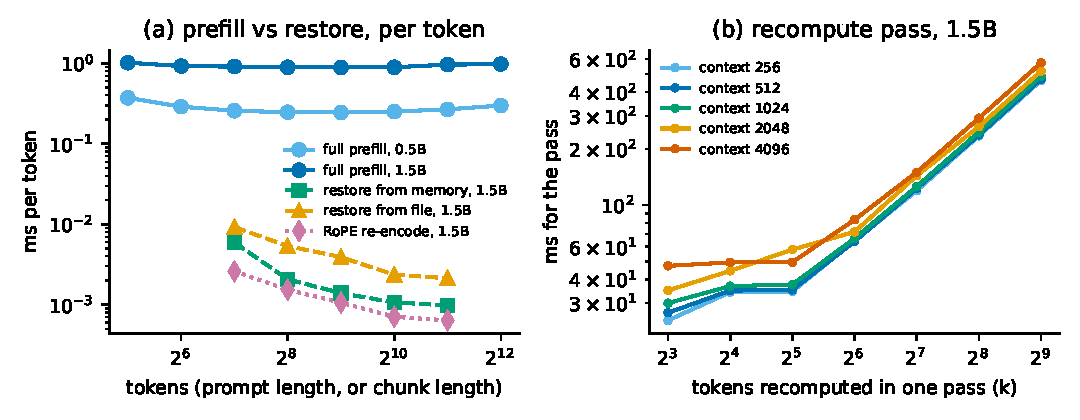
\includegraphics[width=\linewidth]{../figures/fig1_measured_costs.pdf}
\caption{(a) Time per token: full prefill for both models, and restoring a 1.5B chunk from memory, from a warm file,
and the RoPE re-encode pass. (b) One recompute pass on the 1.5B model: time against tokens recomputed, for several
cache sizes. Log axes. Apple M4 laptop, MLX, 4-bit weights.}
\end{figure}

\section{Results - where short contexts fall}
\textbf{Fixed cost per forward call.} A full prefill of 128 tokens takes \preAmsshort{} ms on the 0.5B model and
\preBmsshort{} ms on the 1.5B model. A 32-token prefill takes \preAmsthirtytwo{} ms and \preBmsthirtytwo{} ms. The fitted
fixed cost per call is \constA{} ms and \constB{} ms. For short prompts a large part of the time is this fixed cost, and the
reuse path pays it twice (query pass plus recompute pass), so it cannot win when the reused chunks are small.

\textbf{Restoring is cheap next to computing.} Per token, prefill costs \preAshort{} ms (0.5B) and \preBshort{} ms (1.5B)
at 128 tokens, and \preAlong{} ms and \preBlong{} ms at 2048 tokens. Restoring a 512-token chunk from memory costs
\memA{} and \memB{} ms per token, and from a warm file \fileA{} and \fileB{} ms per token (the 1.5B chunk is
\filembB{} MB). One RoPE pass over a 512-token chunk takes \ropeA{} and \ropeB{} ms in total, and the lookup takes
\lookupA{} and \lookupB{} ms. On this machine the cache-management side is small. Recomputation and the extra call are the
real overhead.

\begin{figure}[h]
\centering
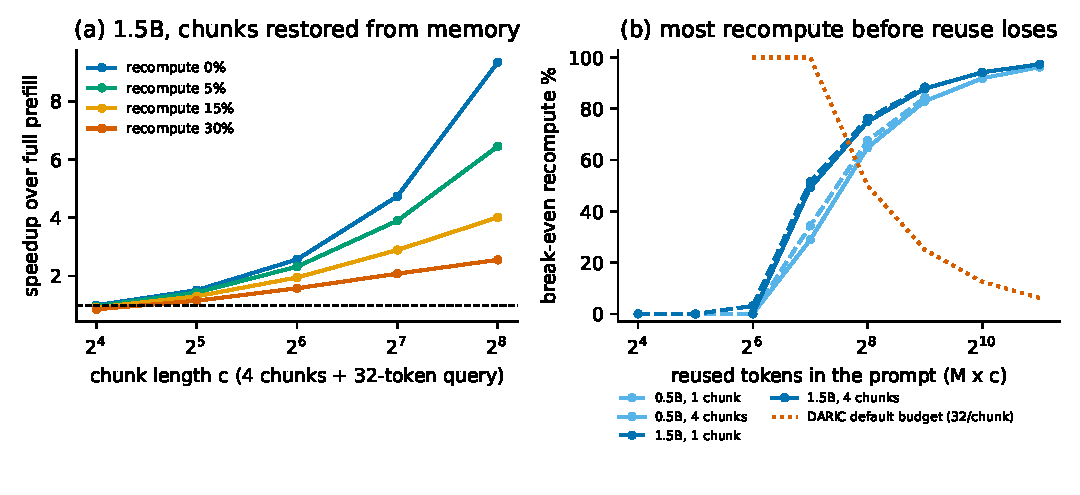
\includegraphics[width=\linewidth]{../figures/fig2_break_even.pdf}
\caption{(a) Fitted speedup of chunk reuse over full prefill for the 1.5B model, 4 reused chunks of 16 to 256 tokens plus a
32-token query, for 0 to 30\% recomputation. Below the dashed line, reuse is slower. (b) Break-even recompute fraction (the most that can be
recomputed before reuse loses) against total reused tokens, for 1 and 4 chunks. The dotted line is the share that DARIC's
default budget of 32 tokens per chunk would take. Chunks restored from memory.}
\end{figure}

\textbf{Break-even.} Table 1 lists the break-even recompute fraction and two speedups from the fitted model, for
short contexts. With 4 chunks on the 1.5B model, the break-even fraction is \beBfourxxxii\% at 32-token chunks,
\beBfourlxiv\% at 64 and \beBfourcclvi\% at 256. At 16-token chunks reuse does not win even with no recomputation. At
15\% recomputation, reuse first beats full prefill at about \crossfifteenA{} reused tokens on the 0.5B model and about
\crossfifteenB{} on the 1.5B model (4 chunks, 32-token query). The bigger model crosses over sooner, because each token
it computes costs more next to the fixed cost of a call.

\begin{table}[h]
\centering\small
\begin{tabular}{lrrrrrr}
\toprule
model & chunks & chunk & break-even & break-even & speedup & speedup\\
 & & length & (memory) & (warm file) & at 15\% & DARIC budget\\
\midrule
0.5B & 1 & 128 & \beAonecxxviii\% & \befileAonecxxviii\% & \sfifteenAonecxxviii x & \sdaricAonecxxviii x\\
0.5B & 4 & 32  & \beAfourxxxii\% & \befileAfourxxxii\% & \sfifteenAfourxxxii x & \sdaricAfourxxxii x\\
0.5B & 4 & 64  & \beAfourlxiv\% & \befileAfourlxiv\% & \sfifteenAfourlxiv x & \sdaricAfourlxiv x\\
0.5B & 4 & 256 & \beAfourcclvi\% & \befileAfourcclvi\% & \sfifteenAfourcclvi x & \sdaricAfourcclvi x\\
1.5B & 1 & 64  & \beBonelxiv\% & \befileBonelxiv\% & \sfifteenBonelxiv x & \sdaricBonelxiv x\\
1.5B & 1 & 128 & \beBonecxxviii\% & \befileBonecxxviii\% & \sfifteenBonecxxviii x & \sdaricBonecxxviii x\\
1.5B & 4 & 32  & \beBfourxxxii\% & \befileBfourxxxii\% & \sfifteenBfourxxxii x & \sdaricBfourxxxii x\\
1.5B & 4 & 64  & \beBfourlxiv\% & \befileBfourlxiv\% & \sfifteenBfourlxiv x & \sdaricBfourlxiv x\\
1.5B & 4 & 256 & \beBfourcclvi\% & \befileBfourcclvi\% & \sfifteenBfourcclvi x & \sdaricBfourcclvi x\\
\bottomrule
\end{tabular}
\caption{Fitted break-even recompute fraction and speedups over full prefill, with a 32-token query. ``DARIC budget''
recomputes 32 tokens per chunk plus the query, which is all of a 32-token chunk, 50\% of a 64-token chunk, 25\% of a
128-token chunk and 12.5\% of a 256-token chunk. Speedups below 1 mean reuse is slower.}
\end{table}

\textbf{Measured check, no fit.} For one 256-token chunk with no query, restore plus one recompute pass of $k$ tokens
was compared directly with the timed 256-token prefill. Recomputing 32 tokens (12.5\%) gave \measAxxxii x (0.5B) and
\measBxxxii x (1.5B). Recomputing all 256 tokens gave \measAcclvi x and \measBcclvi x, so restoring and then recomputing
everything is slightly slower than a plain prefill, as it should be.

\textbf{Forward calls matter.} Folding the query into the recompute pass moves the 1.5B, 4-chunk break-even at 64-token
chunks from \beBfourlxiv\% to \bemergedBfourlxiv\% and the DARIC-budget speedup from \sdaricBfourlxiv x to
\sdaricmBfourlxiv x. For a small model with short chunks, the number of forward calls matters about as much as the number
of recomputed tokens. A fixed per-chunk budget also matters: 32 tokens per chunk is the whole chunk when chunks are
32 tokens long. The paper already uses a smaller budget of 8 tokens per chunk for its short function-calling prompts
(Section 5.2.2).

\section{Limits - what this does not show}
\begin{itemize}\setlength{\itemsep}{1pt}
\item \textbf{Laptop, not phone.} An M4 laptop has more compute and memory bandwidth than a phone, and a phone may need to
keep chunk caches in flash storage rather than RAM. A slower restore lowers the break-even point; slower compute raises it.
Only a run on a phone can say which effect wins there.
\item \textbf{Stand-ins.} Recomputation is timed as $k$ new tokens on top of a cache, not as DARIC's in-place overwrite of
scattered positions. The RoPE pass and the hash lookup are stand-ins for re-encoding and the radix-tree index. The file
read was warm; a cold read from flash would cost more.
\item \textbf{Costs only.} Nothing here measures answer quality, so it cannot say how much recomputation a small model needs.
The paper finds that the needed budget depends on the model and task (Section 5.2.5).
\item \textbf{One machine, batch 1, median of 3 runs}, two models from one family.
\end{itemize}

\section{Takeaway - the short answer}
On this laptop, restoring a chunk's KV cache costs over a hundred times less per token than computing it, so reuse pays
off even for a 0.5B model once the reused part is around a hundred tokens or more. With only a few dozen reused tokens,
the fixed cost of the extra forward call eats the savings even with no recomputation. So for a phone, the first things to check are the cost
per forward call and the cost of reading chunk caches back from storage, more than the recompute budget itself. Code, saved
timings and an interactive version: \url{https://github.com/aarushkandukoori/chunk-reuse-break-even}.

\end{document}
